\documentclass[10pt]{beamer}

\usetheme{metropolis}
\usepackage{appendixnumberbeamer}
\usepackage{booktabs}
\usepackage{listings}
\usepackage{xcolor}
\usepackage{colortbl}
\usepackage{array}
\usepackage{tikz}

% Python listing style
\definecolor{codebg}{HTML}{F5F5F5}
\definecolor{codegreen}{HTML}{28A745}
\definecolor{codepurple}{HTML}{6F42C1}
\definecolor{codeorange}{HTML}{D73A49}
\definecolor{codegray}{HTML}{6A737D}
\lstset{
  language=Python,
  basicstyle=\ttfamily\tiny,
  keywordstyle=\color{codeorange}\bfseries,
  commentstyle=\color{codegray}\itshape,
  stringstyle=\color{codegreen},
  backgroundcolor=\color{codebg},
  frame=single,
  framerule=0.4pt,
  breaklines=true,
  showstringspaces=false,
  columns=fullflexible,
  keepspaces=true,
  tabsize=4,
  xleftmargin=4pt,
  xrightmargin=4pt,
  aboveskip=4pt,
  belowskip=4pt,
  morekeywords={jnp,lax,self,replace},
}

% Green/red highlight for table rows
\definecolor{rowgreen}{HTML}{D4EDDA}
\definecolor{rowred}{HTML}{F8D7DA}
\definecolor{rowyellow}{HTML}{FFF3CD}
\definecolor{rowblue}{HTML}{CCE5FF}

\title{TPU-Specific MXU Amortization\\in Speculative Decoding}
\subtitle{Post-Ablation Experiments \& Research Direction}
\date{Week 7 --- February 22, 2026}
\author{Aaron Feng \and Zhongyan Luo \and Son Nguyen \and Andy Huang}
\institute{UCSD DSC 180 Capstone \quad Mentor: Hao Zhang \quad TA: Yiming Zhao}

\begin{document}

% ============================================================
% Slide 1 -- Title
% ============================================================
\maketitle

% ============================================================
% Slide 2 -- Recap: Where We Left Off
% ============================================================
\section{Recap}

\begin{frame}{Recap: DFlash on TPU}
\begin{block}{What we built (Weeks 1--6)}
Complete port of DFlash speculative decoding from GPU/PyTorch to TPU/JAX.
\end{block}

\centering
\footnotesize
\begin{tabular}{l ccc}
\toprule
& \textbf{TPU v4} & \textbf{GPU (A100)} & \textbf{TPU/GPU} \\
\midrule
$\tau$ (avg) & 6.67 & 7.07 & 94\% \\
Speedup & 3.67$\times$ & 5.53$\times$ & --- \\
TPS & 227 & --- & --- \\
\bottomrule
\end{tabular}

\vspace{0.8em}
\begin{itemize}
  \item \textbf{Algorithmic quality transfers} --- 94\% of GPU $\tau$
  \item \textbf{Speedup gap} ($3.67\times$ vs $5.53\times$) is hardware overhead
  \item \textbf{This week:} What causes the gap? Can we exploit TPU hardware?
\end{itemize}
\end{frame}

% ============================================================
% Slide 3 -- The Pipeline Bottleneck
% ============================================================
\section{Analysis}

\begin{frame}{The Pipeline Bottleneck}
\centering
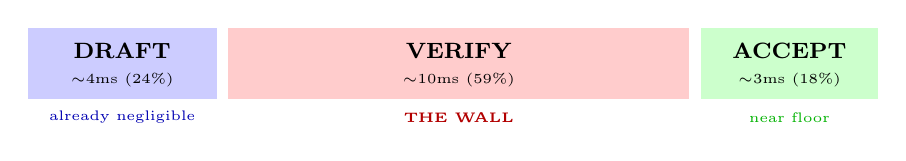
\begin{tikzpicture}[x=0.75cm, y=0.6cm]
  % Draft box
  \fill[blue!20] (0,0) rectangle (3.2,1.5);
  \node[font=\footnotesize\bfseries] at (1.6,1.0) {DRAFT};
  \node[font=\tiny] at (1.6,0.4) {$\sim$4ms (24\%)};

  % Verify box
  \fill[red!20] (3.4,0) rectangle (11.2,1.5);
  \node[font=\footnotesize\bfseries] at (7.3,1.0) {VERIFY};
  \node[font=\tiny] at (7.3,0.4) {$\sim$10ms (59\%)};

  % Accept box
  \fill[green!20] (11.4,0) rectangle (14.4,1.5);
  \node[font=\footnotesize\bfseries] at (12.9,1.0) {ACCEPT};
  \node[font=\tiny] at (12.9,0.4) {$\sim$3ms (18\%)};

  % Labels below
  \node[font=\tiny, text=blue!70!black] at (1.6,-0.4) {already negligible};
  \node[font=\tiny, text=red!70!black] at (7.3,-0.4) {\textbf{THE WALL}};
  \node[font=\tiny, text=green!70!black] at (12.9,-0.4) {near floor};
\end{tikzpicture}

\vspace{0.5em}
\footnotesize
\begin{tabular}{lrl}
\toprule
\textbf{Verify sub-cost} & \textbf{Time} & \textbf{Bottleneck} \\
\midrule
FFN matmuls (36 layers) & $\sim$1.7ms & MXU compute \\
\textbf{Attention (KV cache read)} & \textbf{$\sim$8.3ms} & \textbf{HBM bandwidth} \\
\bottomrule
\end{tabular}

\vspace{0.5em}
Throughput $= \frac{\tau + 1}{T_{\text{step}}} = \frac{7.67}{14\text{ms}} \approx 548$ tok/s (standalone)
\end{frame}

% ============================================================
% Slide 4 -- Key Discovery: MXU Amortization
% ============================================================
\section{Key Discovery}

\begin{frame}{Key Discovery: Verification is Free Up to 256 Tokens}
\begin{alertblock}{Core finding}
On TPU v4, verifying 128 tokens costs the same as verifying 16 tokens.\\
On GPU, verification cost scales linearly with token count.
\end{alertblock}

\centering
\footnotesize
\begin{tabular}{l cccc}
\toprule
\textbf{Query tokens} & \textbf{16} & \textbf{64} & \textbf{128} & \textbf{vs K=16} \\
\midrule
\rowcolor{rowgreen}
TPU verify latency & 1.70ms & 1.69ms & 1.78ms & \textbf{1.05$\times$} \\
\rowcolor{rowred}
GPU verify latency & \multicolumn{4}{c}{\textit{scales linearly (SmartSpec, ICLR 2025)}} \\
\bottomrule
\end{tabular}

\vspace{0.8em}
\textbf{Why?} TPU MXU loads weight matrices from HBM once per layer ($\sim$150 MB).\\
MXU compute for K$\leq$256 finishes within the memory transfer window.\\
\textbf{Operations are memory-bandwidth bound, not compute-bound.}
\end{frame}

% ============================================================
% Slide 5 -- No Tile Boundary Discontinuity
% ============================================================
\begin{frame}{Flat Scaling Extends Beyond K=128}

\textbf{Hypothesis:} Cost should jump at K=129 (second MXU tile row needed).\\
\textbf{Result:} No discontinuity. Flat all the way to K=256.

\centering
\footnotesize
\vspace{0.5em}
\begin{tabular}{r rr rr}
\toprule
& \multicolumn{2}{c}{\textbf{DFlash FFN}} & \multicolumn{2}{c}{\textbf{Target FFN}} \\
\cmidrule(lr){2-3} \cmidrule(lr){4-5}
\textbf{K} & \textbf{ms/layer} & \textbf{vs K=16} & \textbf{ms/layer} & \textbf{vs K=16} \\
\midrule
16  & 0.335 & 1.00$\times$ & 0.339 & 1.00$\times$ \\
64  & 0.328 & 0.98$\times$ & 0.334 & 0.98$\times$ \\
128 & 0.330 & 0.98$\times$ & 0.329 & 0.97$\times$ \\
\rowcolor{rowyellow}
\textbf{129} & \textbf{0.319} & \textbf{0.95$\times$} & \textbf{0.325} & \textbf{0.96$\times$} \\
192 & 0.334 & 1.00$\times$ & 0.341 & 1.00$\times$ \\
256 & 0.343 & 1.02$\times$ & 0.346 & 1.02$\times$ \\
\bottomrule
\end{tabular}

\vspace{0.8em}
\begin{itemize}
  \item K=129/K=128 ratio: \textbf{0.97$\times$} (DFlash), \textbf{0.99$\times$} (Target) --- no step
  \item \textbf{Root cause:} weight loading from HBM dominates; MXU compute for K$\leq$256 is hidden behind memory transfer latency
  \item Design space is wider than expected: K=256 is equally viable
\end{itemize}
\end{frame}

% ============================================================
% Slide 6 -- What We Tried and Ruled Out
% ============================================================
\section{Experiments}

\begin{frame}{What We Tried (Docs 32--35)}
\centering
\footnotesize
\begin{tabular}{l l l c}
\toprule
\textbf{Doc} & \textbf{Experiment} & \textbf{Finding} & \textbf{Viable?} \\
\midrule
32 & Layer truncation & All 36 layers needed; & \textcolor{red}{\textbf{No}} \\
   & & even $-1$ layer $\Rightarrow$ $-30\%$ $\tau$ & \\
\midrule
33 & Amortized verification & Verify(128) $\approx$ Verify(16) & \textcolor{green!60!black}{\textbf{Yes}} \\
   & (microbenchmark) & but multi-block draft overhead kills it & \\
\midrule
34 & TPU vs GPU uniqueness & GPU scales linearly; & \textcolor{green!60!black}{\textbf{Novel}} \\
   & & TPU is flat (MXU-specific) & \\
\midrule
35 & Tree speculation & Each branch +5ms draft; & \textcolor{red}{\textbf{No}} \\
   & (K=1,2,4 branches) & $\tau$ barely improves (+0.5\%) & \\
\bottomrule
\end{tabular}

\vspace{0.8em}
\begin{alertblock}{Pattern}
MXU amortization benefits \textbf{verification}, not drafting.
Any attempt that adds drafting work to fill the verify window negates the gain.
\end{alertblock}
\end{frame}

% ============================================================
% Slide 7 -- Both Sides Amortize
% ============================================================
\begin{frame}{Both Draft and Verify Forward Passes Are Free}

\textbf{Doc 37:} Raw matmul scaling --- drafter also amortizes.

\centering
\footnotesize
\vspace{0.5em}
\begin{tabular}{l ccc}
\toprule
\textbf{Component} & \textbf{K=16} & \textbf{K=128} & \textbf{Ratio} \\
\midrule
\rowcolor{rowgreen}
DFlash FFN (5 layers) & 1.637ms & 1.556ms & \textbf{0.95$\times$} \\
\rowcolor{rowgreen}
Target FFN (36 layers) & 11.871ms & 11.384ms & \textbf{0.96$\times$} \\
\rowcolor{rowgreen}
Attention Q$\times$K$^T$ (KV=256) & 0.202ms & 0.196ms & \textbf{0.97$\times$} \\
\bottomrule
\end{tabular}

\vspace{0.8em}
\begin{columns}[T]
\begin{column}{0.48\textwidth}
\textbf{Implication:}\\
A DFlash retrained with block\_size=128 produces \textbf{8$\times$ more draft tokens} per forward pass at \textbf{zero additional compute cost}.
\end{column}
\begin{column}{0.48\textwidth}
\textbf{Step time budget:}\\[0.3em]
\tiny
\begin{tabular}{lcc}
\toprule
& K=16 & K=128 \\
\midrule
DFlash fwd & 0.36ms & 0.36ms \\
Aux proj & $\sim$2ms & $\sim$2ms \\
Host overhead & $\sim$1.6ms & $\sim$1.6ms \\
Target verify & $\sim$10ms & $\sim$10ms \\
Accept/output & $\sim$3ms & $\sim$3ms \\
\midrule
\textbf{Total} & \textbf{$\sim$17ms} & \textbf{$\sim$17ms} \\
\bottomrule
\end{tabular}
\end{column}
\end{columns}
\end{frame}

% ============================================================
% Slide 8 -- Why DFlash Uses K=16
% ============================================================
\begin{frame}{Why DFlash Uses K=16 (A GPU Constraint)}

\begin{quote}
\footnotesize
``In practical serving scenarios, large blocks can increase verification cost under compute-bound settings; reducing the block size can therefore yield better overall speedup.''\\
\hfill--- \textit{DFlash paper, Section 4.2}
\end{quote}

\vspace{0.5em}
\centering
\footnotesize
\begin{tabular}{l cc}
\toprule
\textbf{Hardware} & \textbf{Verify(128) vs Verify(16)} & \textbf{Optimal K} \\
\midrule
\rowcolor{rowred}
GPU (A100) & $\sim$8$\times$ cost (linear scaling) & K=16 (paper's choice) \\
\rowcolor{rowgreen}
TPU v4 & 1.05$\times$ cost (flat) & K=128+ (free) \\
\bottomrule
\end{tabular}

\vspace{0.8em}
\begin{itemize}
  \item The paper's own ablation shows larger K improves $\tau$ (Table 7: K=16 $\tau$=6.33 vs K=8 $\tau$=5.21)
  \item They chose K=16 because \textbf{GPU verification cost grows with K}
  \item On TPU, this constraint \textbf{does not exist}
  \item K=16 is a \textbf{GPU design parameter}, not an algorithmic optimum
\end{itemize}
\end{frame}

% ============================================================
% Slide 9 -- The Throughput Equation
% ============================================================
\section{Research Direction}

\begin{frame}{How $\tau$ Translates to Throughput}

Step time is constant at $\sim$17ms for any K$\leq$256. Therefore:

$$\text{Throughput} = \frac{\tau + 1}{T_{\text{step}}}$$

\centering
\footnotesize
\vspace{0.3em}
\begin{tabular}{l ccc}
\toprule
\textbf{Scenario} & $\boldsymbol{\tau}$ & \textbf{Throughput} & \textbf{vs current} \\
\midrule
Current (K=16, $\alpha$=0.87) & 6.67 & 548 tok/s & baseline \\
\rowcolor{rowyellow}
K=128, $\alpha$=0.87 (conservative) & 7.69 & 621 tok/s & \textbf{+13\%} \\
\rowcolor{rowgreen}
K=128, $\alpha$=0.90 (improved) & 9.99 & 785 tok/s & \textbf{+43\%} \\
\rowcolor{rowblue}
K=128, $\alpha$=0.93 (optimistic) & 13.29 & 1,021 tok/s & \textbf{+86\%} \\
\bottomrule
\end{tabular}

\vspace{0.8em}
\begin{itemize}
  \item $\alpha$ = per-position acceptance probability (currently 0.87)
  \item $\tau(K) = (1 - \alpha^K) / (1 - \alpha)$ \quad (geometric series)
  \item Conservative case (same $\alpha$): +13\% from longer acceptance chains
  \item \textbf{Key question:} does wider block context improve $\alpha$?
\end{itemize}
\end{frame}

% ============================================================
% Slide 10 -- Why Alpha Might Improve
% ============================================================
\begin{frame}{Why $\alpha$ Might Improve with Wider Blocks}

DFlash uses \textbf{non-causal attention}: each draft position sees all neighbors.

\begin{columns}[T]
\begin{column}{0.48\textwidth}
\textbf{K=16 (current)}
\begin{itemize}
  \item Each position attends to 15 neighbors
  \item Limited within-block context
  \item $\alpha \approx 0.87$
\end{itemize}
\end{column}
\begin{column}{0.48\textwidth}
\textbf{K=128 (proposed)}
\begin{itemize}
  \item Each position attends to 127 neighbors
  \item 8$\times$ richer parallel context
  \item $\alpha \geq 0.87$ (expected)
\end{itemize}
\end{column}
\end{columns}

\vspace{0.8em}
\textbf{Analogy:} Bidirectional models (BERT) outperform left-to-right models on masked prediction because seeing both sides reduces uncertainty. DFlash's non-causal attention is exactly this --- more neighbors $\Rightarrow$ less ambiguity per position.

\vspace{0.5em}
\begin{alertblock}{Key difference from tree/multi-block}
Tree speculation: add drafting work $\propto$ extra tokens (failed, Doc 35).\\
Wide-block: same 0.36ms forward pass, 8$\times$ more tokens, each with richer context.
\end{alertblock}
\end{frame}

% ============================================================
% Slide 11 -- Proposed: TPU-Native Wide-Block DFlash
% ============================================================
\begin{frame}{Proposed: TPU-Native Wide-Block DFlash}

\textbf{Retrain DFlash with block\_size=128 (or 256), optimized for TPU's cost function.}

\vspace{0.5em}
\footnotesize
\begin{tabular}{ll}
\toprule
\textbf{What changes} & \textbf{Detail} \\
\midrule
\texttt{block\_size} & 16 $\rightarrow$ 128 \\
Anchors per sequence & 512 $\rightarrow$ $\sim$48 (3072/128 $\times$ 2) \\
Loss decay $\gamma$ & Retune (more positions before tail shrink) \\
Training data & Reuse 800K samples + cached hidden states \\
Architecture & Unchanged (5 draft layers, shared embed/head) \\
\bottomrule
\end{tabular}

\vspace{0.5em}
\begin{columns}[T]
\begin{column}{0.48\textwidth}
\textbf{Training estimate:}
\begin{itemize}
  \item Trainable params: $\sim$200M
  \item 1--4 days on TPU v4-8
  \item Or: run existing PyTorch code on a single A100 with \texttt{block\_size=128}
\end{itemize}
\end{column}
\begin{column}{0.48\textwidth}
\textbf{What's novel:}
\begin{itemize}
  \item DFlash redesigned for TPU's actual cost function
  \item Eliminates a GPU-specific constraint
  \item Hardware-aware drafter design
\end{itemize}
\end{column}
\end{columns}
\end{frame}

% ============================================================
% Slide 12 -- Two Viable Paths Forward
% ============================================================
\begin{frame}{Two Viable Paths Forward}

\begin{columns}[T]
\begin{column}{0.48\textwidth}
\begin{block}{Path 1: Wide-Block Drafter}
\footnotesize
\textbf{Type:} ML research (retraining)\\[0.3em]
Train DFlash at K=32/64/128/256.\\
Sweep to find optimal K for TPU.\\[0.3em]
\textbf{Expected:} +13\% to +43\% throughput\\
\textbf{Risk:} $\alpha$ may degrade at large K\\
\textbf{Effort:} 1--4 days training
\end{block}
\end{column}
\begin{column}{0.48\textwidth}
\begin{block}{Path 2: Cross-Request Batching}
\footnotesize
\textbf{Type:} Systems engineering\\[0.3em]
Verify B requests' draft tokens together in one target forward pass.\\[0.3em]
\textbf{Expected:} 2--4$\times$ throughput at batch=8\\
\textbf{Risk:} Scheduling complexity\\
\textbf{Effort:} Serving infra changes
\end{block}
\end{column}
\end{columns}

\vspace{0.8em}
\centering
\footnotesize
\begin{tabular}{l cc}
\toprule
& \textbf{Wide-Block} & \textbf{Cross-Request} \\
\midrule
Retraining needed? & Yes & No \\
Infra changes? & No & Yes \\
Single-request benefit? & Yes & No \\
Throughput at batch & Additive & Multiplicative \\
\bottomrule
\end{tabular}
\end{frame}

% ============================================================
% Slide 13 -- Immediate Next Steps
% ============================================================
\begin{frame}{Immediate Next Steps}

\begin{enumerate}
  \item \textbf{GPU comparison benchmark} (ready to run)
    \begin{itemize}
      \footnotesize
      \item Standalone PyTorch script: \texttt{benchmarks/gpu\_matmul\_scaling.py}
      \item Same dimensions, same K values --- direct apples-to-apples
      \item Proves flat scaling is TPU-specific
    \end{itemize}

  \vspace{0.3em}
  \item \textbf{K=128 DFlash training}
    \begin{itemize}
      \footnotesize
      \item Minimal code change: \texttt{block\_size: 16 $\rightarrow$ 128}
      \item Sweep K=32, 64, 128 to measure $\alpha$ vs block width
      \item Can run on existing PyTorch/GPU or port to JAX/TPU
    \end{itemize}

  \vspace{0.3em}
  \item \textbf{Paper writeup}
    \begin{itemize}
      \footnotesize
      \item MXU amortization finding (Docs 33, 34, 37, 39)
      \item DFlash port results (Docs 00--31)
      \item TPU-native drafter direction (Doc 36)
    \end{itemize}
\end{enumerate}
\end{frame}

% ============================================================
% Slide 14 -- Summary
% ============================================================
\section{Summary}

\begin{frame}{Summary}

\begin{block}{Key Finding}
TPU verification cost is \textbf{flat} from 16 to 256 tokens due to memory-bandwidth boundedness. GPU verification scales linearly. This is a hardware-specific property not previously documented.
\end{block}

\begin{block}{What It Means}
DFlash's block\_size=16 is a \textbf{GPU constraint}. On TPU, wider blocks (K=128+) produce more draft tokens at zero additional cost. The optimal drafter design depends on the hardware's cost function.
\end{block}

\begin{block}{What We Ruled Out}
Layer truncation, multi-block speculation, tree speculation --- all fail because draft overhead dominates. The only path is wider blocks with no extra draft passes.
\end{block}

\begin{alertblock}{Open Question}
Does per-position acceptance $\alpha$ improve with wider blocks? A K=128 training sweep answers this and determines the magnitude of the throughput gain (+13\% to +86\%).
\end{alertblock}
\end{frame}

\end{document}
